\documentclass[specialist,
substylefile = spbu_report.rtx,
subf,href,colorlinks=true, 12pt]{disser}

\usepackage[a4paper,
mag=1000, includefoot,
left=3cm, right=1.5cm, top=2cm, bottom=2cm, headsep=1cm, footskip=1cm]{geometry}
\usepackage[T2A]{fontenc}
\usepackage[utf8]{inputenc}
\usepackage[english, russian]{babel}
\ifpdf\usepackage{epstopdf}\fi

\usepackage{bbm}
\usepackage{algorithm}
\usepackage{algpseudocode}
\usepackage{algorithmicx}
\usepackage{amsmath,amssymb,amsthm,amscd,amsfonts}
\usepackage{cmap}
\usepackage{euscript}
\usepackage{mathdots}
\usepackage{graphicx}
\usepackage[russian]{cleveref}

\newenvironment{formulation}{\paragraph{Формулировка.}\itshape}{\hfill}
\newenvironment{corollary}{\paragraph{Следствие.}\itshape}{\hfill}
\newenvironment{remark}{\paragraph{Замечание.}\itshape}{\hfill\\}
\newenvironment{solution}{\paragraph{Решение.}}{\hfill}
% Нумерация подсекций в оглавлении
\setcounter{secnumdepth}{2}

% Включать подсекции в оглавление
\setcounter{tocdepth}{3}

\newcommand{\R}{\mathbb{R}}
\begin{document}
	
	% Название организации
	\institution{%
		Санкт-Петербургский государственный университет \\
		Прикладная математика и информатика \\
		Вычислительная стохастика и статистические модели
	}
	
	% Тема
	\topic{\normalfont\scshape Отчёт по задачам на тему\\«Условные распределения»}
	
	% Автор
	\author{Яковлев Денис Михайлович\\
		Группа 21.Б04-мм\\
		\textsc{st095998@student.spbu.ru}}
	
	% Город и год
	\city{Санкт-Петербург}
	\date{\today}
	
	\maketitle
	\newpage
	\thispagestyle{empty}
	\tableofcontents
	\newpage
	\pagenumbering{arabic}
	\section{Задача 1}
	\begin{formulation}
		Случайные величины $\xi_1,\xi_2,\alpha$ независимы, причём $\xi_1,\xi_2\in N(0,1)$, а $\alpha\in U(0,1)$. Найти распределение случайной величины
		\begin{equation}\label{eqn:1}
			\eta = \dfrac{\xi_1 + \alpha\xi_2}{\sqrt{1+\alpha^2}}.
		\end{equation}
	\end{formulation}
	\begin{solution}
		Итак, поскольку $\xi_1, \xi_2, \alpha$ --- независимые случайные величчины, то их условное распределение будет равносильно безусловному:
		\begin{equation*}
			\rho_{\xi_1,\xi_2,\alpha}(x,y,z)=\rho_{\xi_1}(x)\rho_{\xi_2}(y)\rho_{\alpha}(z).
		\end{equation*}
		Для того, чтобы найти распределение случайной величины $\eta$, заданной равенством \eqref{eqn:1}, проанализируем $\eta$. Заметим, что $\eta$ можно переписать в виде
		\begin{align*}
			&\eta = \xi_1\cos\varphi + \xi_2\sin\varphi,\\
			&\varphi = \arccos\dfrac{1}{\sqrt{1+\alpha^2}}=\arcsin\dfrac{\alpha}{\sqrt{1+\alpha^2}}.
		\end{align*}
		Следовательно, если положить $\alpha=\alpha_0\in(0,1)$, то координаты $\frac{1}{\sqrt{1+\alpha^2}}(\xi_1, \alpha\xi_2)$ будут задавать поворот для координат $(\xi_1, \xi_2),~\xi_1,\xi_2\in N(0,1)$. Так как $\alpha\in U(0,1)$, то $\varphi\in(0, \pi/4)$. Покажем, что $\eta$ не зависит от $\alpha$. Для этого рассмотрим функцию распределения случайной величины $\eta$: 
%		Поскольку поворот не влияет на двумерное нормальное распределение, то параметр $\alpha$ можно зафиксировать произвольным образом. 
%		Положим $\alpha=0$. Тогда
%		\begin{equation*}
%			\eta = \xi_1 \Rightarrow \eta\in N(0,1).
%		\end{equation*}
		\begin{align*}
			&F_\eta(w) = P(\eta<w)=\iiint\limits_{\left \{\dfrac{x + zy}{\sqrt{1+z^2}}<w\right \} }\rho_{\xi_1}(x)\rho_{\xi_2}(y)\rho_{\alpha}(z)~dx~dy~dz\\
			&=\int_0^1\rho_\alpha(z)dz\iint\limits_{\left \{\dfrac{x + zy}{\sqrt{1+z^2}}<w\right \} }\rho_{\xi_1}(x)\rho_{\xi_2}(y)~dx~dy.
		\end{align*}
		Рассмотрим двойной интеграл:
		\begin{equation*}
			\iint\limits_{\left \{\dfrac{x + zy}{\sqrt{1+z^2}}<w\right \} }\rho_{\xi_1}(x)\rho_{\xi_2}(y)~dx~dy
		\end{equation*}
		Как и предполагали ранее, положим $\varphi=\arccos\dfrac{1}{\sqrt{1+z^2}}=\arcsin\dfrac{z}{\sqrt{1+z^2}}$. Тогда при переходе к полярным координатам $(r, \psi)$, используя замену
		\begin{align*}
			&x=r\cos(\psi + \varphi)\\
			&y=r\sin(\psi + \varphi)
		\end{align*}
		и пользуясь тригонометрическими формулами, сведём двойной интеграл к интегралу, характеризующему распределение Рэлея, а именно
		\begin{equation*}
						\iint\limits_{\left \{r<w, \psi\in(0, 2\pi)\right \} }\dfrac{r}{2\pi}e^{-\frac{r^2}{2}}~dr~d\psi.
		\end{equation*}
		Отсюда вытекает, что $\eta\in R(1)$, где $R(1)$ --- распределение Рэлея с дисперсией $\sigma^2 = 1$.
		\begin{corollary}
			В условиях этой задачи, если сохранить независимости случайных величин и положить $\alpha$ произвольным распределением, а $\xi_1, \xi_2 \in N(0, \sigma^2)$, то
			\begin{equation*}
				\eta\in R(\sigma^2).
			\end{equation*}   
		\end{corollary}
		\begin{remark}
			Вышенаписанное сделано с ошибкой: нужно брать интеграл не по всем $\psi\in (0, 2\pi)$.
		\end{remark}
	\end{solution}
	\begin{solution}[Новое решение, с использованием условных распределений.]
		Итак, рассматриваем случайную величину \eqref{eqn:1}. Попробуем посчитать его, используя условные распределение, учитывая, что $\xi_1, \xi_2, \alpha$ --- непрерывные случайные величины. Тогда их условное распределение будет равносильно безусловному:
		\begin{equation*}
			\rho_{\xi_1,\xi_2,\alpha}(x,y,z)=\rho_{\xi_1}(x)\rho_{\xi_2}(y)\rho_{\alpha}(z).
		\end{equation*}
		Вычислим функцию распределения $F_\eta(w)$, пользуясь формулой полных вероятностей:
		\begin{equation}\label{eqn:main}
			F_\eta(w) = P(\eta<w)=\int_\R P(\eta<w~|~\alpha=z)\rho_{\alpha}(z)~dz=\int_0^1 P(\eta<w~|~\alpha=z)~dz.
		\end{equation}
		Теперь вычислим вероятность $P(\eta<w~|~\alpha=z)$.
		\begin{equation*}
			P(\eta<w~|~\alpha=z)=P(\cos(\varphi)\xi_1 + \sin(\varphi)\xi_2 < w).
		\end{equation*}
		Через характеристические функции можно показать, что $\gamma=\cos(\varphi)\xi_1 + \sin(\varphi)\xi_2 \sim N(0,1)$:
		\begin{equation*}
			\varphi_\gamma(x) = Ee^{i\gamma x} = Ee^{i\cos(\varphi)x\xi_1}Ee^{i\sin(\varphi)x\xi_2}=e^{\frac{-\cos^2(\varphi)x^2}{2}}e^{\frac{-\sin^2(\varphi)x^2}{2}}=e^{\frac{-x^2}{2}}.
		\end{equation*}
		Таким образом, из \eqref{eqn:main} получаем
		\begin{equation*}
			F_\eta(w) = P(\eta<w)=\int_0^1 P(\eta<w~|~\alpha=z)~dz=\int_0^1 \Phi(w)~dz = \Phi(w),
		\end{equation*}
		где $\Phi$ --- функция распределения $\xi\sim N(0,1)$. Отсюда,
		\begin{equation*}
			\eta\sim N(0,1).
		\end{equation*}
%		\begin{remark}
%			То, что ниже --- лишнее. Нужно переписать
%		\end{remark}
%		Вычислим функцию распределения $F_\eta(w)$, пользуясь формулой полных вероятностей:
%		\begin{align}
%			&F_\eta(w) = P(\eta<w)=\int_\R P(\eta<w~|~\xi_1=x)\rho_{\xi_1}(x)~dx\nonumber\\
%			&=\iint_{\R^2} P(\eta<w~|~\xi_1=x,\xi_2=y)\rho_{\xi_1}(x)\rho_{\xi_2}(y)~dx~dy\nonumber\\
%			&=\iiint_{\R^3} P(\eta<w~|~\xi_1=x,\xi_2=y,  \alpha=z)\rho_{\xi_1}(x)\rho_{\xi_2}(y)\rho_{\alpha}(z)~dx~dy~dz, \label{eqn:2}
%%			\iiint\limits_{\left \{\dfrac{x + zy}{\sqrt{1+z^2}}<w\right \} }\rho_{\xi_1}(x)\rho_{\xi_2}(y)\rho_{\alpha}(z)~dx~dy~dz\\
%%			&=\int_0^1\rho_\alpha(z)dz\iint\limits_{\left \{\dfrac{x + zy}{\sqrt{1+z^2}}<w\right \} }\rho_{\xi_1}(x)\rho_{\xi_2}(y)~dx~dy.
%		\end{align}
%		где
%		\begin{equation*}
%			P(\eta<w~|~\xi_1=x,\xi_2=y, \alpha=z) =
%			\begin{cases}
%				1,& \dfrac{x + zy}{\sqrt{1+z^2}}<w;\\
%				0,& \dfrac{x + zy}{\sqrt{1+z^2}}\geqslant w;
%			\end{cases}
%		\end{equation*}
%		Таким образом, $P(\eta<w~|~\xi_1=x,\xi_2=y, \alpha=z) = \mathbbm{1}_{\{\frac{x + zy}{\sqrt{1+z^2}}<w\}}(w)$. Тогда можно свести интеграл \eqref{eqn:2} к интегралу
%		\begin{equation*}
%			\iiint\limits_{\left \{\dfrac{x + zy}{\sqrt{1+z^2}}<w\right \} }\rho_{\xi_1}(x)\rho_{\xi_2}(y)\rho_{\alpha}(z)~dx~dy~dz =\int_0^1\rho_\alpha(z)dz\iint\limits_{\left \{\dfrac{x + zy}{\sqrt{1+z^2}}<w\right \} }\rho_{\xi_1}(x)\rho_{\xi_2}(y)~dx~dy. 
%		\end{equation*}
%		Рассмотрим двойной интеграл:
%		\begin{equation*}
%			\iint\limits_{\left \{\dfrac{x + zy}{\sqrt{1+z^2}}<w\right \} }\rho_{\xi_1}(x)\rho_{\xi_2}(y)~dx~dy
%		\end{equation*}
%		Как и предполагали ранее, положим $\varphi=\arccos\dfrac{1}{\sqrt{1+z^2}}=\arcsin\dfrac{z}{\sqrt{1+z^2}}$. Тогда при переходе к полярным координатам $(r, \psi)$, используя замену
%		\begin{align*}
%			&x=r\cos(\psi + \varphi)\\
%			&y=r\sin(\psi + \varphi).
%		\end{align*}
%		Отсюда, получаем
%		\begin{align*}
%			\dfrac{1}{2\pi}\iint\limits_{\left \{r\cos\psi<w, \psi\in(0,2\pi)\right \} }re^{-\frac{r^2}{2}}~dr~d\psi=
%		\end{align*}
	\end{solution}
	\section{Задача 2}
	\begin{formulation}
		Пусть $\xi\in U(0, \sqrt{2})$. В квадрат $(-\xi, \xi)\times(-\xi, \xi)$ бросают точку. Найти совместное распределение её координат.
	\end{formulation}
	\begin{solution}
%		\begin{remark}
%			То, что ниже --- лишнее. Нужно переписать
%		\end{remark}
		Итак, воспользуемся условными вероятностями. Для этого положим $\{\eta_\xi\}$ --- семейство случайных величин с распределением $\eta_\xi \sim U((-\xi, \xi) \times (-\xi, \xi))$. Определим функцию распределения $F_{\eta_\xi}(x, y)$:
		\begin{equation}\label{eqn:main_2}
			F_{\eta_\xi}(x,y) = P(\eta_\xi\in (-\infty, x)\times(-\infty, y))=\int_\R P(\eta_\xi\in(-\infty, x)\times(-\infty, y)~|~\xi=z)\rho_\xi(z)~dz.
		\end{equation}
		Так как $\xi \sim U(0, \sqrt{2})$, то $\rho_\xi(z)=\dfrac{1}{\sqrt{2}},~z\in(0,\sqrt{2})$. При фиксированном $\xi = z$ получаем
		\begin{equation*}
			\rho_{\eta_z}(x,y) = \dfrac{1}{4z^2}\text{ внутри квадрата }(-z,z)\times(-z,z).
		\end{equation*}
		Теперь определим $P(\eta_\xi\in(-\infty, x)\times(-\infty, y)~|~\xi=z)$:
		\begin{align*}
			&P(\eta_\xi\in(-\infty, x)\times(-\infty, y)~|~\xi=z) = \iint\limits_{\{(-z, z)^2\}}\mathbbm{1}_{(-\infty, x)\times(-\infty, y)}(w, u)\dfrac{1}{4z^2}~dw~du\\
			&=\begin{cases}
				0,& x\leqslant-z\text{ или }y\leqslant-z;\\
				(x+z)(y+z)\dfrac{1}{4z^2},&-z<x\leqslant z\text{ и }-z<y\leqslant z;\\
				(x+z)\dfrac{1}{2z},& -z<x\leqslant x \textrm{ и } z<y\\
				(y+z)\dfrac{1}{2z},& z<x \textrm{ и } -z<y\leqslant z\\
				1,& \text{иначе.}
			\end{cases}
		\end{align*}
		При $z \rightarrow0$ считаем, что $U((-z,z)\times(-z,z))\rightarrow \delta_{(0,0)}$. Вычисле
		Таким образом, получаем
% 2-ой вариант.
		Если хотим посчитать функцию распределения в точке $(x,y)$, то необходимо учитывать поведение условного распределения, которое можно разбить на четыре случая в зависимости от того, в какой четверти плоскости располагается $(x,y)$. Например, когда $x<0$ или $y<0$, то 
		\begin{equation*}
			\int_0^{\max\{-x,-y\}}P(\eta_\xi\in (-\infty, x)\times(-\infty, y)~|~\xi=z)~dz = 0,
		\end{equation*}
		поскольку $(-\infty, x)\times(-\infty, y)$ не содержит в себе ни одного квадрата. Когда $x>0$ и $y>0$, то
		\begin{equation*}
			\int_0^{\min\{x,y\}}P(\eta_\xi\in (-\infty, x)\times(-\infty, y)~|~\xi=z)~dz = \min\{x,y\}.
		\end{equation*}
		Для каждой четверти функция распределения будет отличаться по этим соображениям. Тогда получим
		\begin{equation*}
			F_{\eta_\xi}(x,y) = 
			\begin{cases}
				0,& x\leqslant-\sqrt{2} \textrm{ или } y\leqslant-\sqrt{2}\\
				-\dfrac{xy}{8}+\dfrac{x+y}{4\sqrt{2}}\ln\dfrac{\sqrt{2}}{y}+\dfrac{\sqrt{2}-y}{4\sqrt{2}}+\dfrac{x}{4\sqrt{2}}+\dfrac{1}{4}\\+\dfrac{x}{2\sqrt{2}}\ln\dfrac{y}{\min\{-x,y\}}+\dfrac{1}{2\sqrt{2}}(y-\min\{-x,y\}),,&-\sqrt{2}<x\leqslant 0, 0<y\leqslant\sqrt{2}\\
				-\dfrac{xy}{8}+\dfrac{x+y}{4\sqrt{2}}\ln\dfrac{\sqrt{2}}{x}+\dfrac{\sqrt{2}-x}{4\sqrt{2}}+\dfrac{y}{4\sqrt{2}}+\dfrac{1}{4}\\+\dfrac{y}{2\sqrt{2}}\ln\dfrac{x}{\min\{x,-y\}}+\dfrac{1}{2\sqrt{2}}(x-\min\{x,-y\}),&0<x\leqslant\sqrt{2}, -\sqrt{2}<y\leqslant 0\\
				-\dfrac{xy}{8}+\dfrac{x+y}{4\sqrt{2}}\ln\dfrac{\sqrt{2}}{\min\{x,y\}}-\dfrac{|x-y|}{4\sqrt{2}}+\dfrac{1}{4},&-\sqrt{2}<x\leqslant0, -\sqrt{2}<y\leqslant0\\
				\dfrac{\min\{x,y\}}{\sqrt{2}}-\dfrac{xy}{8}+\dfrac{x+y}{4\sqrt{2}}\ln\dfrac{\sqrt{2}}{\min\{x,y\}}+\dfrac{|x-y|}{4\sqrt{2}}+\dfrac{1}{4},&0<x\leqslant\sqrt{2}, 0<y\leqslant\sqrt{2}\\
				1,& \sqrt{2}< x \textrm{ и } \sqrt{2}<y
			\end{cases}
		\end{equation*}
		\begin{remark}
			Громоздкий ответ, который может содержать ошибки.
		\end{remark}
		Чтобы избежать подобных ошибок, упростим задачу и вычислим плотность распределения $\rho_{\eta_\xi}(x,y)$:
		\begin{align}
			&\rho_{\eta_z}(x,y)=\dfrac{1}{4z^2}\mathbbm{1}_{\{(-z,z)^2\}}(x,y);\nonumber\\
			&\rho_{\eta_\xi}(x,y)=\dfrac{1}{\sqrt{2}}\int_{\min\{|x|,|y|\}}^{\sqrt{2}}\rho_{\eta_z}(x,y)dz=(\dfrac{1}{4\sqrt{2}\max(|x|,|y|)} - \dfrac{1}{8})\mathbbm{1}_{\{(-\sqrt{2},\sqrt{2})^2\}}(x,y).\label{eqn:main_prob}
		\end{align}
		Тогда получаем:
		\begin{equation*}
			F_{\eta_\xi}(x,y) = 
			\begin{cases}
				0,& x\leqslant 0 \textrm{ или } y\leqslant 0;\\
				\int_{-\infty}^x\int_{-\infty}^y\rho_{\eta_\xi}(x,y)dz,& \textrm{иначе};\\
				1,& \sqrt{2}<x \textrm{ и } \sqrt{2}<y.
			\end{cases}
		\end{equation*}
% 1-ый вариант
%		Тогда подставим это в \eqref{eqn:main_2} и получим
%		\begin{align*}
%			&F_{\eta_\xi}(x,y) = \dfrac{1}{\sqrt{2}}\int_{\min{|x|,|y|}}^{\sqrt{2}}(x+z)(y+z)\dfrac{1}{4z^2}~dz\\
%			&=\dfrac{1}{4\sqrt{2}}\int_0^{\sqrt{2}}\dfrac{xy}{z^2} + \dfrac{x+y}{z} + 1~dz\\
%			&=...
%		\end{align*}
%		\begin{remark}
%			То, что ниже --- лишнее. Нужно переписать
%		\end{remark}
%		Итак, имеется квадрат с длиной ребра $2\xi$. Введём случайную величину $\eta$, которая имеет распределение на квадрате $S=(-\sqrt{2},\sqrt{2})\times(-\sqrt{2}, \sqrt{2})$, при этом $\eta|\xi=(\eta_1|\xi, \eta_2|\xi)\in U((-\xi, \xi)\times(-\xi, \xi))$. Найдём совместное распределение координат $\eta|\xi$:
%		\begin{equation*}
%			\rho_{\eta|\xi}(x,y|z) = \begin{cases}
%				\dfrac{1}{4z^2},&(x,y)\in(-z,z)\times(-z,z)\\
%				0,& \text{иначе}
%			\end{cases}
%		\end{equation*} 
%		Уточним, что $\eta|\xi$ --- не та случайная величина, для которой мы хотим найти совместное распределение. Мы хотим найти распределение $\eta$, которая уже не зависит от $\xi$. При фиксированном $\xi, \eta|\xi$ --- сечение пирамиды высоты $\sqrt{2}$ с длиной ребра у основания $2\sqrt{2}$ в трёхмерном пространстве
%		\begin{figure}[H]
%			\centering
%			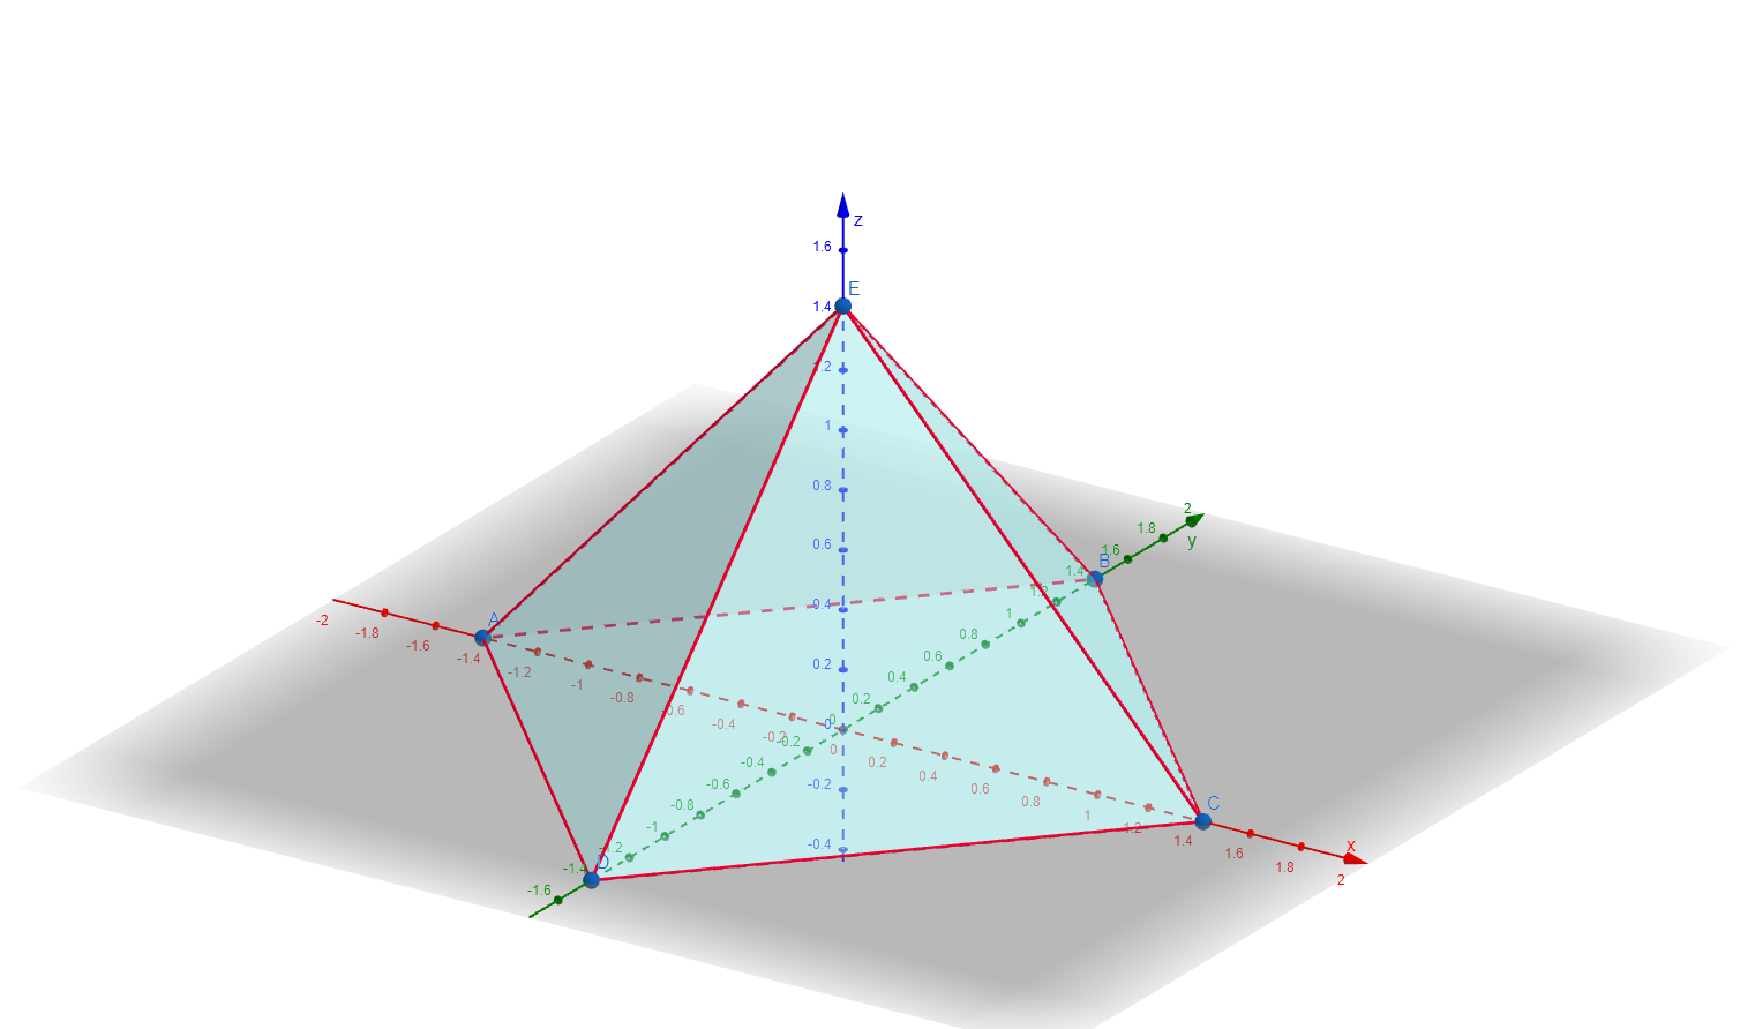
\includegraphics[scale=0.5]{3D Calculator Assignment Sep 13, 2024}
%			\caption{Пирамида}
%		\end{figure} 
%		Графически, чтобы определить плотность распределения $\eta$ в точке $(x,y)$, необходимо сосчитать интеграл плотности распределения от $(x,y,z^*)$ до $(x,y,\sqrt{2})$, где $z^*$ --- значение по оси $Oz$, при котором прямая, перпендикулярная основанию и проходящая через $(x,y,0)$ во второй раз проходит через пирамиду. Воспользуемся тем, что для множества $B_r=\{\max(|x|,|y|)=r\}\quad z^*=\textrm{const}$. \\
%%		Запишем распределение $\eta|\xi$ при $\xi=z$ на некотором множестве $A$:
%%		\begin{equation*}
%%			P(\eta\in A~|~\xi=z)=\dfrac{P(\eta_z\in A)}{\rho_\xi(z)}=\sqrt{2}\iint_A\dfrac{1}{4z^2}~dx~dy
%%		\end{equation*}
%%		Теперь пусть $A=(x,y)\in(-\sqrt{2},\sqrt{2})\times(-\sqrt{2}, \sqrt{2})$. 
%		Пользуясь рассуждением о множестве $B_r$, рассмотрим плотность распределения $\rho_\eta(r)$, пользуясь формулой полных вероятностей. Для нахождения значения $z^*$ положим $y=r$, тогда из подобия треугольников определим длину перпендикуляра $w$:
%		\begin{equation*}
%			\dfrac{\sqrt{2}-r}{\sqrt{2}}=\dfrac{w}{\sqrt{2}}\Rightarrow w = \sqrt{2}-r
%		\end{equation*}
%		Отсюда $z^* = r$. Тогда
%		\begin{equation*}
%			\rho_\eta(r)=\int_\R\rho_{\eta|\xi}(r|z)\rho_\xi(z)~dz= \dfrac{1}{\sqrt{2}}\int_{r}^{\sqrt{2}}\dfrac{1}{4z^2}~dz=\dfrac{1}{4\sqrt{2}r}-\dfrac{1}{8}.
%		\end{equation*}
%		Таким образом, получаем совместную плотность распределения в точке $(x,y)$:
%		\begin{equation*}
%			\rho_\eta(x,y) = \dfrac{1}{4\sqrt{2}\max(|x|,|y|)} - \dfrac{1}{8}.
%		\end{equation*}
%		Теперь найдём функцию распределения для $\eta$:
%		\begin{equation*}
%			F_\eta(x, y) = P(\eta_1<x, \eta_2 < y)=\iint\limits_{\{a<x,b<y\}}\rho_\eta(a,b)~da~db.
%		\end{equation*}
%		Чтобы 
	\end{solution}
\end{document}